\documentclass[]{report}
\usepackage{bookmark}
\usepackage[utf8]{inputenc}
\usepackage{authblk}
\usepackage{amsmath,amsfonts,amsthm,amssymb,mathtools}
\usepackage[english]{babel}


%% theorem, lemma, proof, etc. %%
%% for unnumbed use \newtheorem* and delete section in [---] %%
\newtheorem{theorem}{Theorem}[section]
\newtheorem{corollary}{Corollary}[theorem]
\newtheorem{lemma}[theorem]{Lemma}
\newtheorem{proposition}[theorem]{Proposition}

\theoremstyle{remark}
\newtheorem{remark}{Remark}

\theoremstyle{definition}
\newtheorem{definition}{Definition}[section]

\theoremstyle{definition}
\newtheorem{example}{Example}[section]
%%% theorem %%

\usepackage{enumitem}
\usepackage{graphicx}
\usepackage{subcaption}
\usepackage{tikz}
\usetikzlibrary{decorations.fractals}
\usepackage{float}
\usepackage{dsfont}
\usepackage{geometry}
\geometry{
    a4paper,
    left=30mm,
    right=30mm,
    top=20mm,
    bottom=20mm,
}

%%%% hyperref %%%%
\usepackage{url}
\usepackage{hyperref} % for link
\hypersetup{
    colorlinks=true,
    allcolors=black,
}
\usepackage{cleveref}
%%% fancyhdr %%%% for footer and Hader of document
\usepackage{fancyhdr}
%\pagestyle{fancy}
%\lhead{lest hand head} %% left Hader %%
%\rhead{Measure Theory} %% right Hader %%
\cfoot{\thepage} %% central footer %%

\setlength{\headheight}{14.49998pt}

%% for code 
\usepackage{xcolor}
\usepackage{tcolorbox}
\usepackage{listings}
\lstset{language=Python,
        basicstyle=\ttfamily\small,
        %% keywordstyle=\color{blue},
        commentstyle=\color{black},
        %% stringstyle=\color{orange},
        showstringspaces=false,
        breaklines=true,
        frame=single,
        %% numbers=left,
        %% numberstyle=\tiny\color{gray}
}

%%% spacing in document %%%
\usepackage{setspace}
\onehalfspacing

\title{Markov Chain}
\author{Azmain Biswas}
\date{April 2023}

\begin{document}

\begin{titlepage}
    \thispagestyle{empty}
    \begin{center}

        \vspace{3cm}

        \Large{A Project Report\\ on}\\
        \huge{\textbf{Markov Chain And It's Applications}}

        \vspace{2cm}

        \large{{in the partial fulfillment of the requirements for the award of the degree of}}\\
        \Large{\textbf{M.Sc. in Applied Mathematics}}\\ 
        \large{\textbf{by}}\\ 
        \Large{\textbf{Azmain Biswas}}\\ 
        \large{\textbf{Enrollment No.: 2022MAM008}}\\ 
        \Large{Under the supervision of}\\ 
        \Large{\textbf{Prof. M. Mitra}}

        \vspace{2cm}

        
\includegraphics[scale = 0.09]{pic/IIEST_Shibpur_Logo.svg.png}

        \vspace{1cm}

        \Large{{
                INDIAN INSTITUTE OF ENGINEERING SCIENCE AND TECHNOLOGY, Shibpur\\ 
                \textbf{Department of Mathematics}
        }}

        \vspace{3cm}

        \large{DECLARATION: I affirm that I have identified all my sources and that no part of my dissertation paper uses unacknowledged materials.}
    \end{center}
    \large{SIGNATURE:}
\end{titlepage}

\vspace{10cm}
\begin{center}
    \LARGE{\textbf{CERTIFICATE}}
\end{center}

\vspace*{2cm}
This is to certify that the Term Paper on \textbf{"Markov Chains and their Applications"} submitted by Azmain Biswas to the Department of Mathematics, Indian Institute of Engineering Science and Technology, Shibpur, Howrah-711103, for 2nd semester of Master of Science in Applied Mathematics is a record of project work carried out by him under my supervision. \\
The result of this project work or any part thereof has not been submitted for any degree or diploma.
\vspace{4cm}
\begin{flushright}
    Prof. M. Mitra\\
    Department of Mathematics\\
    Indian Institute of Engineering Science and Technology\\
    Shibpur, Howrah.
\end{flushright}

\vspace{2cm}
\begin{center}
    \LARGE{\textbf{Acknowledgment}}
\end{center}
\vspace{2cm}
    Thanks to my supervisor, Prof. M. Mitra, for a very interesting project. It has been a great pleasure to work under his guidance, and I have learned a lot from his way of thinking and his approach to a problem. 
    \vspace{0.2cm}

    I am also indebted to Prof. Pritha Das the Head of the Department of Mathematics, Indian Institute of Engineering Science and Technology, Shibpur, for his help and inspiration. 
    
    \vspace{0.2cm}
    At various stages, I received encouragement and inspiration for most of the faculty members of the departiment. I would like to thank all of them for their invaluable words of advice, and the interest they have taken in my work.

    \vspace{0.2cm}
    I have benefited greatly from the advantages of the TEX-group software typing systems, the use of which has contributed much to simplify the typing of long mathematical expressions involved in my work.

    \vspace{0.2cm}
    I would like to thank my parents and friends, for being so supportive of my career and life choices, as well as for making me happy.

    \vspace{2cm}
    \begin{flushright}
        Azmain Biswas
    \end{flushright}

\tableofcontents

\newcommand{\cosec}{\operatorname{cosec}}
\newcommand{\tx}[1]{\text{#1}}
\newcommand\numberthis{\addtocounter{equation}{1}\tag{\theequation}}

\chapter{Introduction}
The Weak law of large number(WLLN) and the Central Limit theorem(CTL) proved around  1880's. At that time those were the focal probabilistic issues.
In 1902 Russian Mathematician cum Philosopher P.A. Nekrasov claimed that pairwise independent of random variables were necessary condition for CTL to hold. 
This motivated Andrei A. Markov to construct a counterexample to disprove the claim of P.A. Nekrasov. So He developed Markov Chain in 1907 to disprove a 
"Mathematical proof of freewill" which had been proposed by P.A.Nekrasov to defend the church.

 A Markov chain is a stochastic model that describes a sequence of possible
events or transitions from one state to another of a system. The probability of transitions
from state to state only depends on the current state of the system. A Markov Chain is
used to unravel predictions about future states of a stochastic process using only knowledge
of the present state. This property of “forgetting” past states is known as the memoryless
property.

Now a days Markov Chain is a very important concept, it is used in various fields like computer science, mathematics, physics, economics, and more.
Markov chains have proven to be an effective modelling and analysis method for systems that change over time.


\chapter{Markov Chain}

\section{Definition}

\begin{definition}[Markov Chain]
    A discrete time stochastic process $\{X_n,n=1,2,3,\ldots\}$ is defined to be \textit{Discrete Time Markov Chain} or simply \textit{Markov Chain}
    if it takes value  the state space $ \mathbf{S} $, and for every
    $n\ge 0$ it satisfy the property
    \begin{equation}
        \label{Markov property}
         \mathbf{P}( X_{n+1} = j | X_n =i , X_{n-1} = i_{n-1}, \ldots, X_0 = i_0 ) = \mathbf{P}( X_{n+1} = j | X_n =i )
    \end{equation}
\end{definition}

Unless otherwise mentioned we take the state space $ \mathbf{S} $ to be $\{0, 1, 2, 3, \ldots\ \} $. 
If $X_n = i $ we say that the process is in $i $th state at time $n$.
In the definition \cref{Markov property} may be interpreted as for Markov Chain, the conditional distribution of any future state $ X_{n+1} $, given the past states  $ X_0, X_1,\ldots, X_{n-1} $  and the present state $ X_n $, is independent of the past and only depend on the present state.
This property is called \textit{Markovian Property}. In other word for Markov chain predicting the future we only need information about the present state.

\textbf{Note:} Assumption we are making for Markov chain to forget the past as long as present in known is very strong assumption.

\section{Homogeneous Markov Chain}

\begin{definition}[Homogeneous Markov Chain]
    We say a Markov chain $ \{ X_n,n\ge 0 \} $ is homogeneous if $ \mathbf{P}(X_{n+1}=j|X_n=i)=\mathbf{P}(X_2=j|X_1=i) \ \forall n>0 $. 
\end{definition}

The quantity $ \mathbf{P}(X_{n+1}=j|X_n=i) $ is called the \textit{transition probability} from state $i$ to state $j$. For homogeneous Markov Chain 
we can specify the transition probabilities $ \mathbf{P}(X_{n+1}=j|X_{n}=i) $ by a sequence of value $ p_{ij} = \mathbf{P}(X_{n+1}=j|X_{n}=i) $.

Then the transition probabilities are $ p_{ij}, $ 
$ 1\le i,j \le \infty $ for transition from state i to state j. The matrix  $ P = (p_{ij}) $ is called The
\textit{Transition Matrix} of chain. Since probabilities are nonnegative and since the process must make a transition into some state, we have
\[
    p_{ij}\ge 0,\ \ i,j\ge 0,\ \text{and } \sum_{j=0}^{\infty}p_{ij} = 1,\ \  \forall\ i=0,1,2,\ldots.
\]

For, infinite state Markov chain the probability transition matrix will be infinite order. 
Then,
\[
    P = 
    \begin{bmatrix}
        p_{00} & p_{01} & p_{02} & \ldots \\
        p_{10} & P_{11} & p_{12} & \ldots \\
        \vdots & \vdots & \vdots & \ldots \\ 
        p_{i0} & \ldots & p_{ij} & \ldots \\
        \vdots & \vdots & \vdots & \ddots 
    \end{bmatrix}
\]

\begin{example}[Rain and sunny]
    Suppose that whether it rains today depends on previous weather conditions only from the last two days. 
    Specifically, suppose that if it has rained for the past two days, 
    then it will rain tomorrow with probability 0.7; 
    if it rained today but not yesterday, then it will rain tomorrow with probability 0.5; 
    if it rained yesterday but not today, then it will rain tomorrow with probability 0.4; 
    if it has not rained in the past two days, then it will rain tomorrow with probability 0.2.
    
    We can transform it into a Markov chain by letting the state on any day be determined by the weather conditions during both that day and 
    the preceding one. For instance, we can say that the process is in

    \begin{center}
        State 0: if it rained both today and yesterday\\ 
        State 1: if it rained today but not yesterday\\ 
        State 2: if it rained yesterday but not today\\ 
        State 3: if it rained neither today nor yesterday 

    \end{center}

    The it will be 4-state Markov chain whose transition matrix will be,
    \[
        P=
        \begin{bmatrix} 
            0.7 & 0 & 0.3 & 0 \\ 
            0.5 & 0 & 0.5 & 0 \\ 
            0 & 0.4 & 0 & 0.6 \\ 
            0 & 0.2 & 0 & 0.8
        \end{bmatrix} 
    \]
\end{example}

\section{Chapman-Kolmogorov Equations}
We have already defined the one step transition probabilities $ p_{ij} $. We now define the n-step transition probabilities $ p_{ij}^{n} $ 
to be the probability that a process in state $i$ will be in state $j$ after $n$ additional transitions. i.e.
\[
    p^{n}_{ij}=\mathbf{P}(X_{n+m}=j|X_{m}=i), \ n\ge 0, \ i,j\ge 0.
\]

By definition of Markov chain we get,
\begin{align*}
    p_{ij}^{n+m} &= \mathbf{P}(X_{n+m}=j|X_{0}=i) \\ 
                 &= \sum_{k=0}^{\infty}\mathbf{P}(X_{n+m}=j,X_{n}=k|X_{0} = i)\text{ (By theorem of total probability)} \\
                 &= \sum_{k=0}^{\infty}\mathbf{P}(X_{n+m}=j|X_{n}=k,X_{0} = i)\mathbf{P}(X_{n}=k|X_{0}=i) \\
                 &= \sum_{k=0}^{\infty}\mathbf{P}(X_{n+m}=j|X_{n}=k)\mathbf{P}(X_{n}=k|X_{0}=i) \\
\end{align*}
Then,
\begin{align*}
     p_{ij}^{n+m} = \sum_{k=0}^{\infty}p_{kj}^{m}p_{ik}^{n}. \numberthis \label{Chapman-Kolmogorov equation} \\
\end{align*}
If we take $ n=m=1 $. Then
\begin{equation}
    \label{2-step probability}
    p_{ij}^{2} = \sum_{k=0}^{\infty} p_{kj}p_{ik}
\end{equation}
the above expression is $ (i,j) $ element of $ P^{2} $ matrix then we see \cref{2-step probability} in matrix form,
\[
    P^{2}=P\cdot P
\]
Hence, \cref{Chapman-Kolmogorov equation} can also written in matrix form,
\[
    P^{n+m}=P^{n}\cdot P^{m}
\]
Where $ P^{n}\ \text{ and } P^{m} $ are the $n$-step and $m$-step transition matrix respectively.

\begin{example}[Transition matrix of 4-state Markov chain]
    Consider the 4-state
    Markov chain depicted in Fig \ref{4-step transition matrix example} When no probabilities are written over the
    arrows, as in this case, it means all arrows originating from a given state are equally
    likely. For example, there are 3 arrows originating from state 1, so the transitions
    $1 \to 3$, $1 \to 2$, and $1 \to 1$ all have probability 1/3. Therefore, the transition matrix of the chain is.

    \begin{figure}[ht]
        \centering
        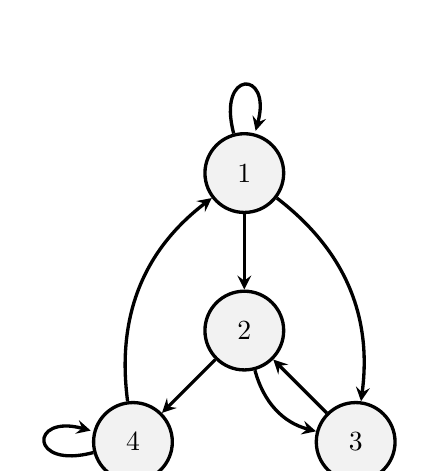
\begin{tikzpicture}[->, >=stealth, auto, very thick, node distance = 2cm, state/.style={circle, draw=black, fill=black!5, very thick, minimum size = 10mm}]
            \node[state] (1) {$1$};
            \node[state] (2) [below of=1] {$2$};
            \node[state] (3) [below right of=2] {$3$};
            \node[state] (4) [below left of=2] {$4$};

            \path (1) edge [loop above] (1)
                (1) edge []  (2)
                (1) edge [bend left] (3)
                (2) edge [bend right] (3)
                (2) edge [] (4)
                (3) edge [] (2)
                (4) edge [bend left] (1)
                (4) edge [loop left] (4);
        \end{tikzpicture}
        \caption{Example of a 4-state Markov chain}
        \label{4-step transition matrix example}
    \end{figure}

    \[
        P=
        \begin{bmatrix}
            \frac{1}{3} & \frac{1}{3} & \frac{1}{3} & 0 \\
            0 & 0 & \frac{1}{2} & \frac{1}{2} \\ 
            0 & 1 & 0 & 0 \\ 
            \frac{1}{2} & 0 & 0 & \frac{1}{2} 
        \end{bmatrix}
    \]
    To compute the probability that the chain is in state 3 after 5 steps, starting at
    state 1, we would look at the (1,3) entry of $ P^{5} $.
    \[
        P^5 =
        \begin{bmatrix}
            \frac{853}{3888} & \frac{509}{1944} & \frac{52}{243} & \frac{395}{1296} \\
            \frac{173}{864} & \frac{85}{432} & \frac{31}{108} & \frac{91}{288} \\
            \frac{37}{144} & \frac{29}{72} & \frac{1}{9} & \frac{11}{48} \\
            \frac{499}{2592} & \frac{395}{1296} & \frac{71}{324} & \frac{245}{864} \\
        \end{bmatrix}
    \]
    so, $ p^{5}_{13}=\mathbf{P}(X_{5}=3|X_{0}=1) = \frac{52}{243} $.
\end{example}

To get the marginal distributions of $X_0, X_1,...$ , we need to specify not just the
transition matrix, but also the initial conditions of the chain. This can be done by
setting the initial state $X_{0}$ to be a particular state, or by randomly choosing $X_0$
according to some distribution. Let $(t_1, t_2,...,t_N)$ be the PMF of $X_{0}$ displayed as
a vector, that is, $t_i = \mathbf{P}(X_0 = i)$. Then the marginal distribution of the chain at any time can be computed from the transition matrix.

\begin{proposition}[Marginal Distribution of $ X_{n} $]
    Define $ \mathbf{t} = (t_{1}, t_{2}, \ldots, t_{n})$ by $ t_{i}=\mathbf{P}(X_{0}=i) $, and view $ \mathbf{t} $ as a row vector.
    Then the marginal distribution of $ X_{n} $ is given by the vector $ \mathbf{t}P^{n} $. That is the $ j $-th component of  $ \mathbf{t}P^{n} $ 
    is $ \mathbf{P}(X_{n}=j) $.
\end{proposition}
\begin{proof}
    By the law of total probability we get,

    \begin{align*}
        \mathbf{P}(X_{n}=j) &= \sum_{i=0}^{N} \mathbf{P}(X_{n},X_{0}=i)\\
                            &= \sum_{i=0}^{N} \mathbf{P}(X_{0}=i)\mathbf{P}(X_{n}=j|X_{0}=i)
    \end{align*}

    \begin{equation*}
                                    = \sum_{i=0}^{N} t_{i}p^{n}_{ij}
    \end{equation*}
    Which is the $ j $-th component of  $ \mathbf{t}P^{n} $.
\end{proof}

\begin{example}[Marginal distribution of 4-state Markov chain]
    Again consider the 4-state Markov chain in Fig. \ref{4-step transition matrix example}. 
    Suppose the initial conditions are $ \mathbf{t} = (1/4,1/4,1/4,1/4) $, Let $ X_{n} $ be the position of the chain at time $ n $. 
    Then distribution of  $ X_{1} $ is
    \begin{align*}
        \mathbf{t}P &= \begin{bmatrix} \frac{1}{4} & \frac{1}{4} & \frac{1}{4} & \frac{1}{4} \end{bmatrix} 
        \begin{bmatrix}
            \frac{1}{3} & \frac{1}{3} & \frac{1}{3} & 0 \\
            0 & 0 & \frac{1}{2} & \frac{1}{2} \\ 
            0 & 1 & 0 & 0 \\ 
            \frac{1}{2} & 0 & 0 & \frac{1}{2} 
        \end{bmatrix}\\
                    &= \begin{bmatrix} \frac{5}{24} & \frac{1}{3} & \frac{5}{24} & \frac{1}{4} \end{bmatrix} 
    \end{align*}
    The marginal distribution of $ X_{5} $ is 
    \begin{align*}
        \mathbf{t}P^{5} &= \begin{bmatrix} \frac{1}{4} & \frac{1}{4} & \frac{1}{4} & \frac{1}{4} \end{bmatrix}
        \begin{bmatrix}
            \frac{853}{3888} & \frac{509}{1944} & \frac{52}{243} & \frac{395}{1296} \\
            \frac{173}{864} & \frac{85}{432} & \frac{31}{108} & \frac{91}{288} \\
            \frac{37}{144} & \frac{29}{72} & \frac{1}{9} & \frac{11}{48} \\
            \frac{499}{2592} & \frac{395}{1296} & \frac{71}{324} & \frac{245}{864} \\
        \end{bmatrix}\\
                        &= \begin{bmatrix}
                            \frac{707}{3254} & \frac{472}{1619} & \frac{101}{486} & \frac{1469}{5184}
                        \end{bmatrix} \\
    \end{align*}
\end{example}

\section{Classification of states}
\begin{definition}[]
    We say that state $j$ is \textit{accessible} from state $i$, written as $ i \to j $, If  $ p^{n}_{ij}>0 $ for some $ n\ge 0 $.\\ 
    We assume every state is accessible from itself since
    \[
        p^{0}_{ii} = \mathbf{P}(X_{0}=i|X_{0}=i) = 1.
    \]
\end{definition}

\begin{definition}[]
    Two states $i$ and $j$ are said to \textit{communicate} , written as $ i \longleftrightarrow j $, if they are accessible from each other.\\ 
    i.e.
    \[
        i\longleftrightarrow j \implies i \to j \ \And j\to i
    \]
\end{definition}

Communication is an equivalence relation. That means that,
\begin{enumerate}
    \item $ i\longleftrightarrow i $,
    \item if $ i\longleftrightarrow j $ then  $ j\longleftrightarrow i$,
    \item if  $ i\longleftrightarrow j $ and  $ j\longleftrightarrow k $ then  $ i\longleftrightarrow k $.
\end{enumerate}

First two properties are obvious from definition, let for some $n,\ m \ge 0$ then, $ p^{n}_{ij},\ p^{m}_{jk}>0 $ by assumption.
By Chapman-Kolmogorov equatation.
\[
    p^{n+m}_{ik} = \sum_{r=0}^{\infty} p^{n}_{ir}p^{m}_{rk} \ge p^{n}_{ij}p^{m}_{jk}>0.
\]
Hence state k is accessible from state i. By same one can prove that $i$ is also accessible from $K$.

Therefore, the states of a Markov chain can be partitioned into communicating classes such that 
only members of the same class communicate with each other. 
i.e. two states $ i \ \&\ j $ belong to same class if and only if $ i\longleftrightarrow j $.

\begin{example}[]
    Consider the markov chain define in the picture \cref{example of communication}.
\begin{figure}[h]
    \centering
    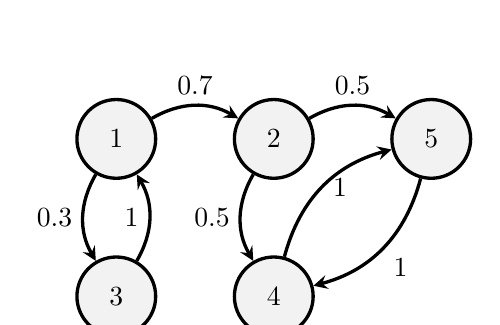
\begin{tikzpicture}[->, >=stealth, auto, very thick, node distance = 2cm, state/.style={circle, draw=black, fill=black!5, very thick, minimum size = 10mm}]
        \node[state] (1) {$1$};
        \node[state] (2) [right of=1] {$2$};
        \node[state] (3) [below of=1] {$3$};
        \node[state] (4) [below of=2] {$4$};
        \node[state] (5) [right of=2] {$5$};

        \path (1) edge [bend right] node [left] {0.3} (3)
              (1) edge [bend left] node [above] {0.7} (2)
              (3) edge [bend right] node {1} (1)
              (2) edge [bend right] node [left] {0.5} (4)
              (2) edge [bend left] node {0.5} (5)
              (4) edge [bend left] node [right] {1} (5)
              (5) edge [bend left] node {1} (4);
    \end{tikzpicture}
    \caption{Communication classes}
    \label{example of communication}
\end{figure}

here the classes are $\{ 1,3 \}, \{2\}, \{4,5\}$
\end{example}

\begin{definition}[Irreducible Markov chain]
    A Markov chain is said to be irreducible if it has only one communicating class. That is, every state communicate with each other.\\ 
    That is, for any states $i$, $j$ there is some positive integer $n$ such that the $(i, j)$ entry of $ P^{n} $ is positive.
\end{definition}

A Markov chain that is not irreducible called reducible.

For any state $ i $ and $ j $ define $ f^{n}_{ij} $ to be the probability that, starting from $ i $, the first transition into $ j  $
occurs at $ n $ time. \\ 
i.e. 
\[
    f^{n}_{ij} = \mathbf{P}(X_{n},X_{k}\neq j, k=1,2,\ldots n-1|X_{0}=i).
\]
Let
\[
    f^*_{ij}=\sum_{n=0}^{\infty} f^{n}_{ij}
\]

Then, $ f^*_{ij} $ denote the probability of ever making a transition into step $ j $ when start from state $ i $. 
If $ j $ is not accessible from $ i $ then $ f^*_{ij} $ will be zero.

\begin{definition}[Recurrent and Transient state]
    A state $ j $ of a Markov chain is said to be \textit{recurrent}  $ f^*_{ii}=1 $ and \textit{transient}  if $ f^*_{ii}<1 $.
\end{definition}

In other word, if a Markov chain start in a recurrent state, there is a guarantee that it will visit that state again in the future
(eventually return to that state with probability 1).

In contrast, a transient state in a Markov chain is a state where, once you reach it, 
there is a positive probability that you will never return to that state.
i.e. if you begin in a transient state, there's a chance you won't return there.

\begin{corollary}
    \label{recurrent}
    state $ i $ is recurrent if and only if  $ \sum_{n=0}^{\infty} p^{n}_{ii}=\infty $
\end{corollary}
\begin{proof}
    The state $ i $ is recurrent if and only if, starting in state  $ i $, the expected number of time periods that the 
    process is in state  $ i $ is infinite. \\ 
    Let
    \[
        I_{n} =
        \begin{cases}
            1, \ \ &\text{if}\ X_{n} = i\\ 
            0, \ \ &\text{if}\ X_{n} \neq  i\\ 
        \end{cases}
    \]
    we then have $ \sum_{n=0}^{\infty} I_{n} $ represent the number of periods that the process is in state $ i $ Then,

    \begin{align*}
        E\left[\sum_{n=0}^{\infty} I_{n}|X_{0}=i\right]&= \sum_{n=0}^{\infty} E[I_{n}|X_{0}=i] \\
        &= \sum_{n=0}^{\infty} \mathbf{P}(X_{n}=i|X_{0}=i) \\
        &= \sum_{n=0}^{\infty} p^{n}_{ii} 
    \end{align*}
    Hence the result.
\end{proof}

\begin{theorem}[]
    \label{recurent if communicate}
    If $ i $ is recurrent and $ i\longleftrightarrow j $, then  $ j $ is also recurrent.
\end{theorem}
\begin{proof}
    Let $ m $ and  $ k $ be such that  $ p^{k}_{ij}>0,p^{m}_{ji}>0 $. Now for any $ n\ge 0 $
    \[
        p^{m+n+k}_{jj}\ge p^{m}_{ji}p^{k}_{ii}p^{m}_{ij}
    \]
    This follows because the left-hand side of the preceding equation is the probability of going $j \to j$ in $m+n+k$ steps,
      whereas the right-hand side is the probability of going $j \to j$ in $m+n+k$ steps
      via a path that goes from $j \to i$ in $m$ steps, then $i \to i$ in $n$ additional steps,
      then $i \to $j in $k$ additional steps. By summing the preceding over n. we obtain
    \[
        \sum_{n=0}^{\infty} p^{m+n+k}_{jj}\ge p^{m}_{ji}p^{k}_{ii} \sum_{n=0}^{\infty}  p^{n}_{ij} = \infty
    \]
     where $ \sum_{n=0}^{\infty}  p^{n}_{ij} = \infty $ because state $ i $ is recurrent. Thus, $j$ is also recurrent.
\end{proof}

\begin{proposition}
     In an irreducible Markov chain with a finite state space, all states are recurrent.
\end{proposition}

\begin{definition}[Absorbing State]
    A state $ i $ of Markov chain is called absorbing it  $ p_{ii} = 1 $ that is, it is impossible to leave 
    the state. 
\end{definition}

A Markov Chain is absorbing if it has at least one absorbing state.

For example consider the Markov chain shown in Fig. \ref{Absorving markov chain}

\begin{figure}[H]
    \centering
    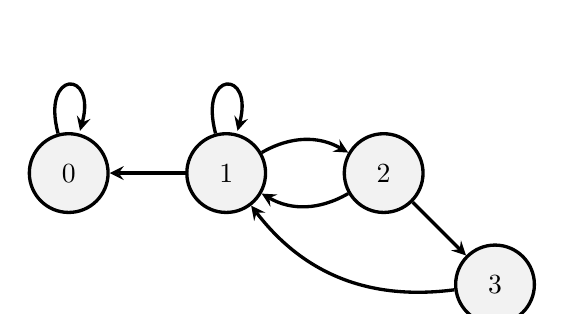
\begin{tikzpicture}[->, >=stealth, auto, very thick, node distance = 2cm, state/.style={circle, draw=black, fill=black!5, very thick, minimum size = 10mm}]
        \node[state] (0) {0};
        \node[state] (1) [right of=0] {1};
        \node[state] (2) [right of=1] {2};
        \node[state] (3) [below right of=2] {3};

        \path (0) edge [loop above] (0)
        (1) edge [] (0)
        (1) edge [loop above] (1)
        (1) edge [bend left] (2)
        (2) edge [bend left] (1)
        (2) edge [] (3)
        (3) edge [bend left] (1);
    \end{tikzpicture}
    \centering
    \caption{Absorbing Markov Chain}
    \label{Absorving markov chain}
\end{figure}

here $p_00=1$ hence, State 0 is Absorbing State in this case.

\chapter{Stationary Probability}
Consider a two-state Markov chain with transition probability matrix 
\[
    P=
    \begin{bmatrix} 
        0.35 & 0.65\\ 
        0.89 & 0.11
    \end{bmatrix} 
\]
Then 2-step transition matrix will be 
\[
    P^{2} = 
    \begin{bmatrix}
        0.7010  &  0.2990 \\ 
        0.4094  &  0.5906 
    \end{bmatrix} 
\]
Then 8-step transition matrix will be
\[
    P^{8} = 
    \begin{bmatrix}
        0.5810  &  0.4190\\ 
        0.5737  &  0.4263 
    \end{bmatrix} 
\]
Once again 12-state transition matrix is,
\[
    P^{12} = 
    \begin{bmatrix}        
        0.5782  &  0.4218\\ 
        0.5776  &  0.4224
    \end{bmatrix} 
\]
Note that The 8-step transition matrix is almost identical to 12-step transition matrix. So it seems that  $ p^{n}_{ij} $ is converging to some
value as $ n\to \infty $ that is same for all $ i $. In other words, In other word it seems to exist a limiting probability that the process will be 
in state  $ j $ after a large number of transitions, and this value is independent of initial state. This limiting probability is known as 
stationary probability and the distribution  of $ X_{j}^{n} $ as $ n\to \infty $ is known as stationary distribution.

State $ i $ is said to have  \textit{period} $ d $ if $ p^{n}_{ii} = 0 $ whenever $ n $ is not divisible by  $ d $, and  $ d $ is the largest
integer with this property. A state with period 1 is said to be \textit{aperiodic}. We denote period of $ i $ by $ d(i) $.

If state $i$ is recurrent, then it is said to be positive recurrent if, starting in state the expected time until the process returns to state $i$ 
is finite. While there exist recurrent states that an not positive recurrent (such states are
called null recurrent). Postie recurrent, aperiodic states are called \textit{ergodic}.

\begin{definition}[Stationary Distribution]
    \label{Stationary distribution}
    A probability distribution $ \{p_{j},j\ge 0\} $ is called stationary for the Markov chain if 
    \begin{equation}
        \label{1st stationary distribution}
        p_{j} = \sum_{i=0}^{\infty} p_{i}p_{ij},\ j \ge 0
    \end{equation}
    i.e. If $ \mathbf{t}=(p_{1},p_{2},\ldots,p_{j},\ldots) $ is a probability distribution vector and $ P $ is transition matrix, Then
    \begin{equation}
        \label{stationary distribution matrix}
         \mathbf{t}=\mathbf{t}P.
    \end{equation}
\end{definition}

From \cref{stationary distribution matrix} we see that 1 is a eigenvalue of transition matrix $ P $ and  $ \mathbf{t} $ is eigenvector corresponding
to 1. Since in transition matrix  such that  $ \sum_{j=0}^{\infty} p_{ij} = 1\ \forall i$ i.e. sum of all elements of row is 1,
1 must be a eigenvalue.

Now the question aeries is eigenvector corresponding to 1 is a probability vector(sum of all component in 1) or not.

\begin{theorem}[Existence and Uniqueness of Stationary Distribution]
    An irreducible aperiodic Markov chain belongs to one of the following two classes:
    \begin{enumerate}
        \item Either the state are all transient or all null recurrent; in this case $ P^{n}_{ij}\to 0 $ as $ n\to \infty \ \forall i,j $
            and there exist no stationary distribution.
        \item Or else, all states are positive recurrent, i.e.
            \[
                \pi_{j} = \lim_{n\to \infty}p_{ij}^{n}>0.
            \]
            In this case, $ \{\pi_{j},j=0,1,\ldots\} $ is stationary distribution and there exist no other stationary distribution.
    \end{enumerate}
\end{theorem}
\begin{proof}
    we will first proof (2),
    we have,
    \[
        \sum_{j=0}^{M} p^{n}_{ij} \le \sum_{j=0}^{\infty} p^{n}_{ij} =1 \ \forall M.
    \]
    Letting $ n\to \infty $ we get,
    \begin{align*}
        \sum_{j=0}^{M} &\pi_{j}\le 1 \ \forall M.\\ 
        \sum_{j=0}^{\infty} &\le 1.
    \end{align*}
    Now, 
     \[
         p^{n+1}_{ij} = \sum_{k=0}^{\infty} p^{n}_{ik}p_{kj}\ge \sum_{k=0}^{M} p_{ik}^{n}p_{kj} \ \forall M.
    \]
    Letting $ n\to \infty $ gives us,
    \[
        \pi_{j}\ge \sum_{k=0}^{M} \pi_{k}p_{kj} \ \forall M,
    \]
    i.e.
    \[
        \pi_{j}\ge \sum_{k=0}^{\infty} \pi_{k}p_{kj}, \ \forall j\ge 0.
    \]
    To show that the above is actually an equality, suppose the inequality is strict for some $ j $. Then we obtain,
     \[
        \sum_{j=0}^{\infty} \pi_{j}> \sum_{j=0}^{\infty} \sum_{k=0}^{\infty} \pi_{k} p_{jk} = \sum_{k=0}^{\infty} \pi_{k}\sum_{j=0}^{\infty} p_{kj} = \sum_{k=0}^{\infty} \pi_{k}.
    \]
    which is contradiction. Therefore,
    \[
        \pi_{j}=\sum_{k=0}^{\infty} \pi_{k}p_{kj}, \ \ \forall j,\ldots
    \]
    Potting $ p_{j}=\pi_{j}/\sum_{0}^{\infty} \pi_{k} $, we see that $ \{p_{j},j=0,1,2,\ldots\} $ is stationary distribution, and hence at least one 
    stationary distribution exist. Now let $ \{p_{j},j=0,1,2,\ldots\} $ be any stationary distribution. Then if $ \{p_{j},j=0,1,2,\ldots\} $ is the probabolity
    distribution of $ X_{0} $ then 
    \begin{align*}
        p_{j} &= \mathbf{P}(X_{n}=j) \\
        &= \sum_{i=0}^{\infty} \mathbf{P}(X_{n}=j|X_{0}=i)\mathbf{P}(X_{0}=i) \\
        &= \sum_{i=0}^{\infty} p^{n}_{ij}p_{i} \numberthis \label{4.3.2}
    \end{align*}
    Then, from \cref{4.3.2} we see,
    \[
        p_{j}\ge \sum_{i=0}^{M}p^{n}_{ij}p_{i} \ \ \forall M.
    \]
    Letting $ n $ and then $ M $ approach $ \infty $ we get,
    \[
        p_{j}\ge \sum_{i=0}^{\infty} \pi_{j}p_{i} = \pi_{j}.
    \]
    Now we show that $ p_{j}\le \pi_{j} $ use \cref{4.3.2} and that fact that $ p _{ij}^{n}\le 1 $ to obtain
    \[
        p_{j}\le \sum_{i=0}^{M} p^{n}_{ij}p_{i} + \sum_{i=M+1}^{\infty} p_{i} \ \forall M.
    \]
    and letting $ n\to \infty $ gives,
    \[
        p_{j}\le \sum_{i=0}^{M} \pi_{j}p_{i} + \sum_{i=M+1}^{\infty} p_{i} \ \forall M.
    \]
    Since $ \sum_{0}^{\infty} = 1 $, we obtain upon letting $ M\to \infty $ that
    \begin{equation}
        p_{j}\le \sum_{i=0}^{\infty} \pi_{j}p_{i} = \pi_{j}.
    \end{equation}

    If the state are transient or null recurrent and $ \{p_{j},j=0,1,2,\ldots\} $ is a stationary distribution, then \cref{4.3.2} hold and $ p_{ij}^{n}\to 0 $,
    which is clearly impossible. Thus, for case (1), no stationary distribution exists and the proof is complete. 
\end{proof}

\chapter{Some Example of Markov Chain}
\section{The Simple Random Walk}
The markov chain whose state space is the set of all integers $ \mathds{Z} $ and has transition probabilites
\[
    p_{i,i+1} = p = 1-p_{i,i-1}, \ \ i\in\mathds{Z}.
\]
where $ 0<p<1 $, is called the simple random walk.

\begin{figure}[h]
    \centering
    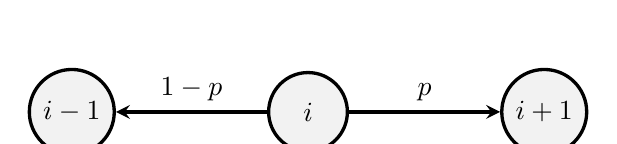
\begin{tikzpicture}[->, >=stealth, auto, very thick, node distance = 3cm, state/.style={circle, draw=black, fill=black!5, very thick, minimum size = 10mm}]
        \node[state] (1) {$i$};
        \node[state] (2) [right of=1] {$i+1$};
        \node[state] (3) [left of=1] {$i-1$};

        \path (1) edge [] node {$p$} (2)
            (1) edge [] node[above] {$1-p$} (3);
    \end{tikzpicture}
    \caption{Simple Random Walk}
    \label{Simple random walk}
\end{figure}

One interpretation is that it represents the winnings of a gambler who on each play of the game either wine or loses one dollar.

Since all state clearly communicate it follows that from \cref{recurent if communicate} they are either all transient or all recurrent. 
So let us consider state 0 and
attempt to determine if  $ \sum_{n=0}^{\infty} p_{00}^{n} $ if finite or not.

Since it is impossible to be back at the initial state after an odd number of transition, we must have,
\[
    p^{2n+1}_{00} = 0 \ \forall \ge 0.
\]

On other hand, the gambler would be even after $ 2n $ trials if and only if he wens  $ n $ games and lost  $ n $ of games.
It is like coin toss with probability of getting head is $ p $ ans tail in  $ 1-p $. Then the desired probability is those binomial probability.
Then we have,
 \[
     p^{n}_{00} = \binom{2n}{n}p^{n}(1-p)^{n} = \frac{2n!}{n!n!}(p(1-p))^{n}, \ \ n=1,2,3,\ldots
\]
by using an starling approximation,
i.e.
\[
    n! \sim \sqrt{2\pi n}\left(\frac{n}{e}\right)^{n}.
\]
we obtain 
\[
    p^{2n}_{00}\sim \frac{[4p(1-p)]^{n}}{\sqrt{n\pi}}
\]
we know if $ a_{n}\sim b_{n} $, then $ \sum_{n}a_{n}<\infty  $ iff $ \sum_{n}b_{n}<\infty  $. Consequently $ \sum_{n}p^{n}_{00}<\infty  $ 
if and only if
\[
    \sum_{n=0}^{\infty} \frac{[4p(1-p)]^{n}}{\sqrt{n\pi}} < \infty
\]

However, $ 4p(1-p)\le 1 $ with equality holding if and only if $ p=\frac{1}{2} $. Hence $ \sum_{n=1}^{\infty} p^{n}_{00}=\infty $ 
if and only if $ p=\frac{1}{2} $. Thus, the chain is recurrent with $ p=\frac{1}{2} $ and transient when  $ p\neq \frac{1}{2} $.

Hence if $ p= 1/2 $ then the process random walk visit state 0 again and again infinitely many time and if  $ p \neq 1/2 $ it may or may 
not visit state 0.

If we consider random walk has  $ N+1 $ step i.e.  $ \{0,1,\ldots,N\} $ is state space of random walk.
Then, The transition matrix will be.
\[
    P = 
    \begin{bmatrix}
        1-p & p & 0 & 0 & \ldots\\ 
        1-p & 0 & p & 0 & \ldots\\ 
        0 & 1-p & 0 & 1-p & \ldots\\ 
        \vdots & \vdots & \vdots & \vdots & \ddots
    \end{bmatrix}_{(N+1)\times(N+1)}
\]
considering $ p_{00} = 1-p $ and $ p_{N N} = p $ as those are last state.

\begin{example}
    Consider a random walk with 4 state and $ p = 0.6 $.\\ 
    Then, the transition probability will be,
    \[
        P = 
        \begin{bmatrix}
            0.4 & 0.6 & 0 & 0\\ 
            0.4 & 0 & 0.6 & 0\\ 
            0 & 0.4 & 0 & 0.6\\ 
            0 & 0 & 0.4 & 0.6
        \end{bmatrix} 
    \]
    then 10000-step transition probability will be
    \[
        P^{10000}=
        \begin{bmatrix}
            0.1231 & 0.1846 & 0.2769 & 0.4154 \\
            0.1231 & 0.1846 & 0.2769 & 0.4154 \\
            0.1231 & 0.1846 & 0.2769 & 0.4154 \\
            0.1231 & 0.1846 & 0.2769 & 0.4154 \\
        \end{bmatrix}
    \]
    hence, Stationary distribution will be 
    \[
        \pi = 
        \begin{bmatrix}
            0.1231 &   0.1846  &  0.2769  &  0.4154
        \end{bmatrix} 
    \]
    As, $ \pi = \pi P $
\end{example}

\subsection{Random Walk in Python}
We can visualize Random Walk with the help of python.

\begin{figure}[htpb]
    \centering
    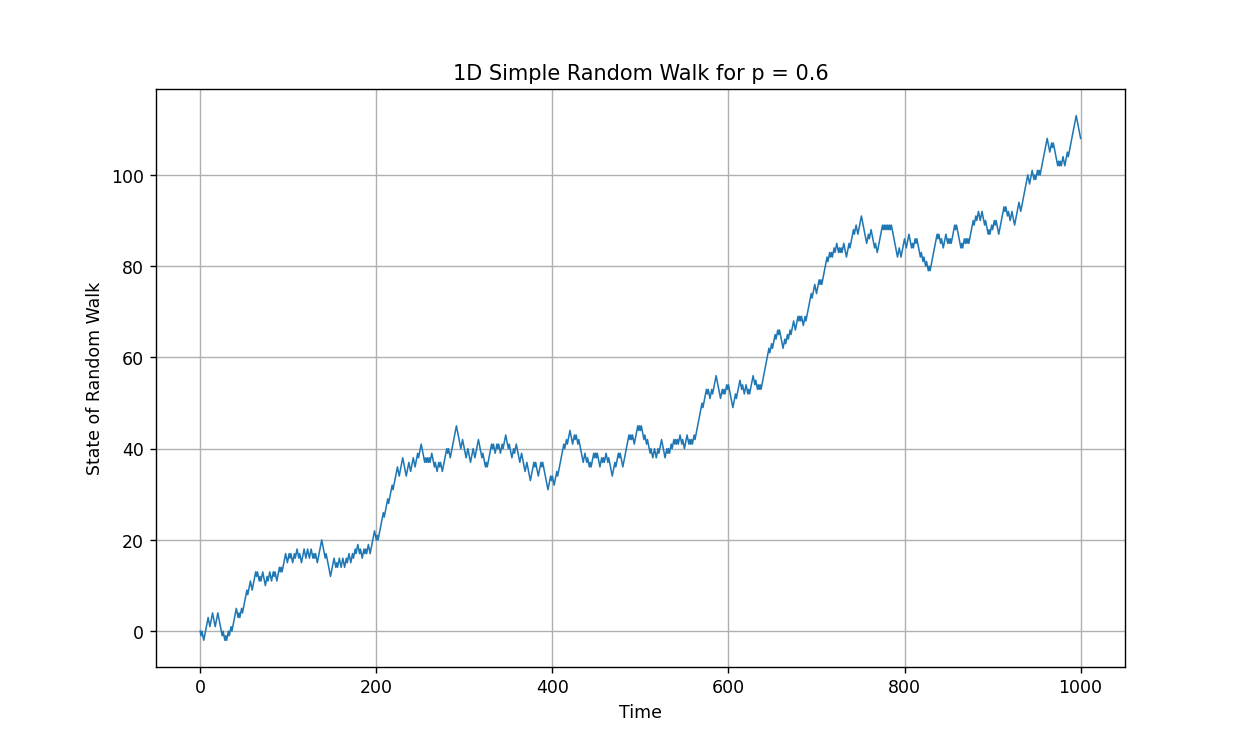
\includegraphics[width=0.7\textwidth]{pic/Random_Walk_0.6.png}
    \caption{Random Walk for $p=0.6$}
    \label{fig:0.6}
\end{figure}
\begin{figure}[htpb]
    \centering
    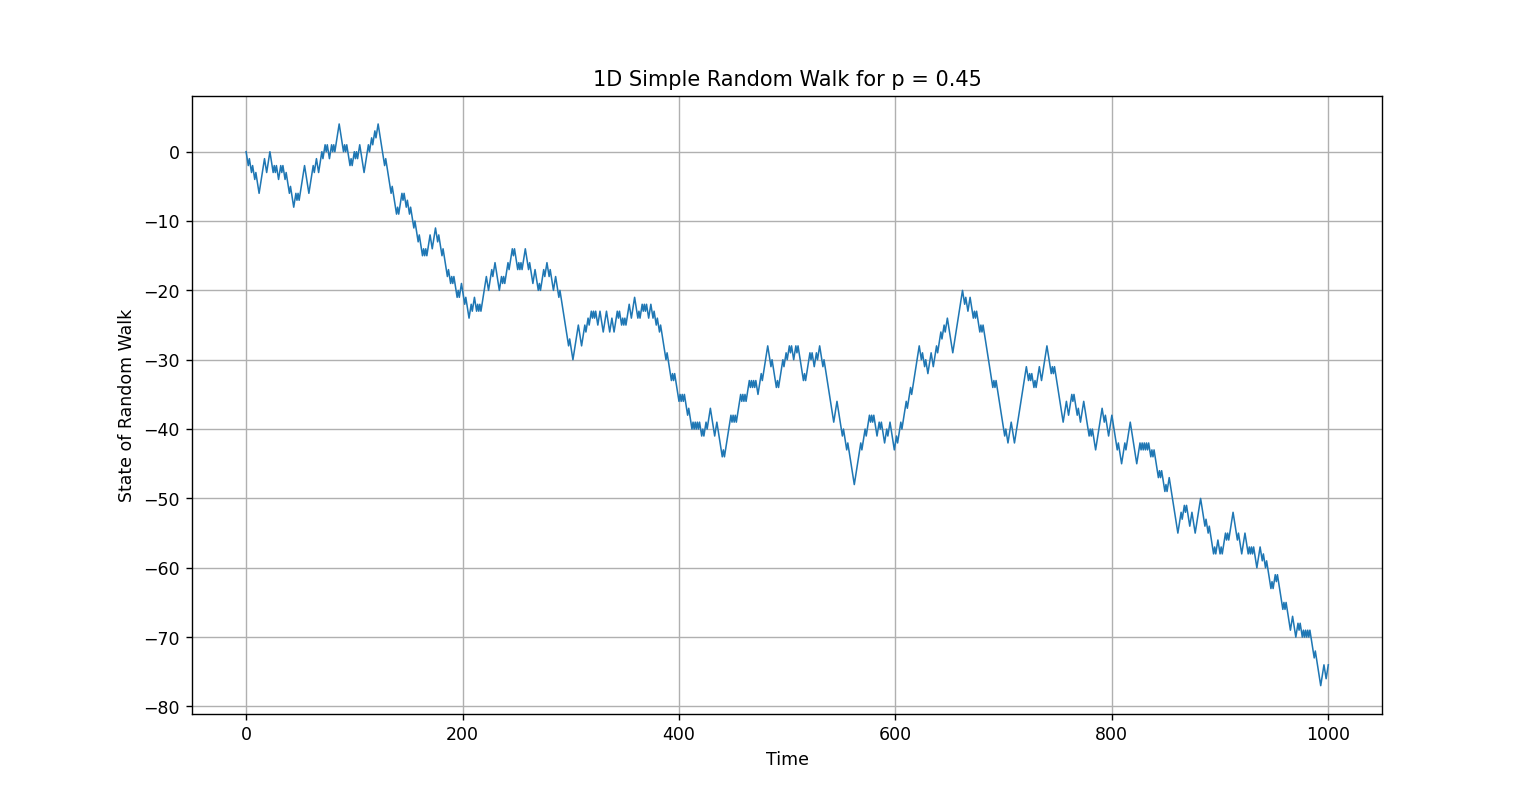
\includegraphics[width=0.7\textwidth]{pic/Random_Walk_0.45.png}
    \caption{Random Walk for $p=0.45$}
    \label{fig:0.45}
\end{figure}
\begin{figure}[htpb]
    \centering
    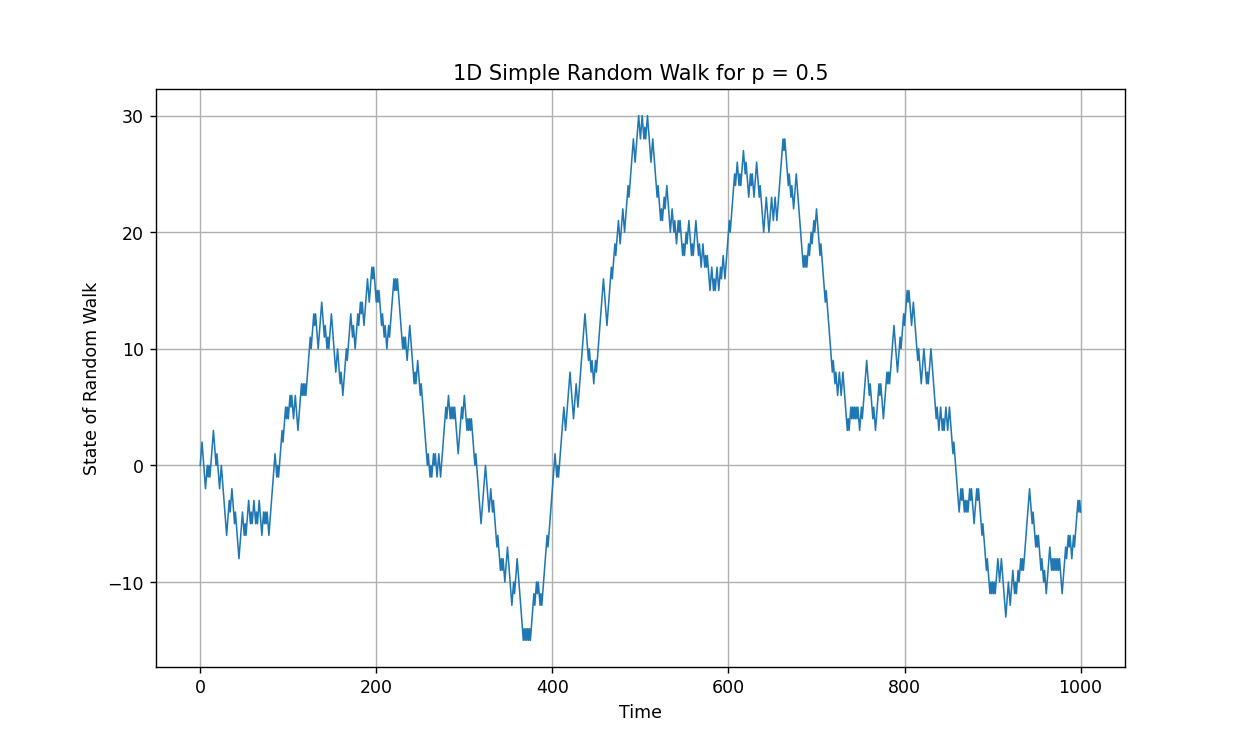
\includegraphics[width=0.7\textwidth]{pic/Random_Walk_0.5.png}
    \caption{Random Walk for $p=0.35$}
    \label{fig:0.5}
\end{figure}

\newpage
\begin{centering}
    \textbf{Code:}
\begin{lstlisting}
    import numpy as np
    import matplotlib.pyplot as plt
    # define number of steps and starting point
    NumberOfStape = 1000
    start = 0
    p = 0.5 # probability of going up.
    Prob = [ p, 1 - p ]
    Position = [ start ]
    Step = [ 1, -1 ]
    for i in range(NumberOfStape):
    rr = np.random.random()
    if rr < Prob[0]:
    position = Position[-1] + 1
    else:
    position = Position[-1] -1
    Position.append(position)
    # for ploting Random Walk
    fig = plt.figure(figsize=(10,6), dpi=125)
    plt.plot(Position, linewidth=0.7)
    plt.xlabel("Time")
    plt.ylabel("State of Random Walk")
    plt.title("1D Simple Random Walk")
    plt.grid(True)
    plt.show()
\end{lstlisting}
\end{centering}

\section{The Gambler's Ruin Problem}
Consider a gambler who starts with an initial fortune and then on each successive gamble
either wins $\$1$ or loses $\$1$ independent of the past with probabilities $p$ and $q = 1-p$ respectively.
The gambler’s objective is to reach a total fortune of $\$N$, without first getting ruined (running out of money). If the gambler succeeds,
then the gambler is said to win the game. In any case, the gambler stops playing after winning
or getting ruined, whichever happens first. Let the gambler starts with $\$i$ where $0 < i < N$.

Let $X_{n}$ denote the total fortune after the $n$th gamble. Then $X_{0}=i$, \\
Then the process $ \{X_{n},n=0,1,2,\ldots,N\} $ is a Markov chain With 
transition probabilities
\begin{align*}
    p_{00} &= p_{N N} = 1,\\ 
    p_{i,i+1} &= p = 1-p_{i,i-1} \ \ i=1,2,\ldots,N-1
\end{align*}

This Markov chain has three classes, classes are $ \{0\},\ \{1,2,\ldots,N-1\}\ \&\ \{N\} $ the first and third class being recurrent and 
second transient. Since all each transient state is only visited finitely often, it follows that after some finite amount of time, the gambler
will either wins $ \$N $ or go broke.

Since the game stops when either $X_{n} = 0$ or $X_{n} = N$, let
\[
    \tau_{i} = \min{n\ge 0: X_{n}\in\{0,N\}|X_{0}=i} 
\]
denote the time at which the game stops when $ X_{0} = i $. If $ X_{\tau_{i}} = N $, then the gambler wins of $ X_{\tau_{i}} = 0 $ gambler is ruin.

Let $ P_{i} = \mathbf{P}(X_{\tau_{i}} = N) $ denotes the probability that the gambler wins when $ X_{0} = i $ clearly $ P_{0} = 0 $ and $ P_{N} = 1 $ 
by definition, (Here $ f_{00}=1  $ and $ f_{N N}=1 $ then state 0 and $ N $ is absorbing state.) 
we next proceed to compute $P_i$, $1 \le  i \le  N - 1$. By conditioning on the outcome of the initial play of the game, we obtain,
\[
    P_{i} = pP_{i+1} + qP_{i-1}, \ \ i=1,2,\ldots,N-1,
\]
Since, $ p + q = 1 $ we get, 
\begin{align*}
    pP_{i} + qP_{i} &= pP_{i+1} + qP_{i-1}\\ 
    P_{i+1} - P_{i} &= \frac{q}{p}(P_{i}-P_{i-1}), \ \ 0<i<N,
\end{align*}
In particular, $ P_{2}-p_{1}=(q/p)(P_{1}-P_{0})=(q/p)P_{1} $ (since, $ P_{0} = 0 $) So that,\\ 
$ P_{3}-P_{2}=(q/p)(P_{2}-P_{1}) = (q/p)^{2}P_{1}$, And hence,
\begin{equation*}
    P_{i+1} -P_{i} = \left( \frac{q}{p} \right)^{i}P_{1}\ \  0<i<N.
\end{equation*}

\begin{align*}
    P_{i+1} -P_{1} &= \sum_{k=1}^{i} (P_{k+1}-P_{k})\\ 
    P_{i+1} -P_{1} &= \sum_{k=1}^{i}\left(\frac{q}{p}\right)^{k}P_{1}  \\
    P_{i+1} &= P_{1} + \sum_{k=1}^{i}\left(\frac{q}{p}\right)^{k}P_{1} =  P_{1}\sum_{k=0}^{i}\left( \frac{q}{p} \right) \\
            &=  \begin{cases}
                P_{1}\frac{1-\left(\frac{q}{p}\right)^{i+1}}{1-\left(\frac{q}{p}\right)} \ \text{ if } p\neq q;\\ 
                P_{1}(i+1) \ \text{ if } p=q=0.5
            \end{cases} \numberthis \label{1st recurtion}
\end{align*}

Choosing $ i=N-1 $ we get and using  $ P_{N} =1 $ we get,
\[
    1=P_{N}=
    \begin{cases}
        P_{1}\frac{1-\left(\frac{q}{p}\right)^{N}}{1-\left(\frac{q}{p}\right)} \ \text{ if } p\neq q;\\ 
        P_{1}N \ \text{ if } p=q=0.5
    \end{cases}
\]
Hence we get, $ P_{1} = 1/N $ when $ p=q=0.5 $ and  $ P_{1} = \frac{1-(q/p)}{1-(q/p)^{N}} $ Then,
\[
    P_{i}=
    \begin{cases}
        \frac{1-(\frac{q}{p})^{i}}{1-(\frac{q}{p})^{N}}, \ \text{ it } p\neq q;\\ 
        \frac{i}{N} \ \text{ if } p=q=0.5 
    \end{cases} \numberthis \label{probability of ruin or win}
\]

\subsection{Becoming infinitely rich or getting ruined}
If $ p>0.5 $, Then  $ \frac{q}{p}<1 $ from \cref{probability of ruin or win} we get,
\[
    \lim_{N \to \infty} P_{i} = 1-\left(\frac{q}{p}\right)^{i} >0 
\]
i.e. if $ p>0.5 $, there is a positive probability that the gambler will never get ruined but instead will become infinitely rich as $ N\to \infty $.

If $p\le 0.5$ then $ \frac{q}{p}\ge 1 $ thus from \cref{probability of ruin or win}
\[
    \lim_{N \to \infty} P_{i} = 0, \ \ \ p\le 0.5
\]
i.e. if $p \le 0.5$ (each gamble is not in his favor), then with probability one the gambler will get ruined $ N\to \infty $.

\begin{example}[Random walk hitting probabilities]
    Ellen bought a share of stock for $\$10$, and it is believed that the stock price moves (day by day) 
    as a simple random walk with $p = 0.55$. What is the probability that Ellen’s
    stock reaches the high value of $\$15$ before the low value of $\$5$? 

    What is the probability that Ellen will become infinitely rich?
\end{example}

\textbf{Solution: } Let us define,
$ P(a) = \mathbf{P}\left(X_{n} \text{ hits }a \text{ before hitting } b\right)$ 

We want calculate the probability that the stock goes up by 5 before going down by 5.

By letting $ a=5 $ and $ b=5 $ and $ N=a+b=10 $, we can imagine a gambler who started with $ \$5 $ and want to win $ \$5 $
before going broke. So we can compute $P(a)$ by casting the problem into the framework of the gamblers ruin problem: 
$ P(a) = P_{5} $ and $ N=10 $. Then,
\[
    P(5) = P_{5} = \frac{1-\left(\frac{0.45}{0.55}\right)^{5}}{1-\left(\frac{0.45}{0.55}\right)^{10}} = \frac{1-(0.82)^{5}}{1-(0.85)^{10}} = 0.73
\]

To see Ellen will ever be infinity rich we make  $ N\to\infty $ and started gamblers ruin problem at $ \$10 $ then,
\[
    \lim_{N\to\infty}P_{10} = 1 - (q/p)^{10} = 1 - (0.82)^{10} = 0.86
\]


\subsection{Gambler's Ruin Problem in python}
We can nicely make a simulation of Gambler's ruin problem.


\begin{figure}[H]
    \centering
    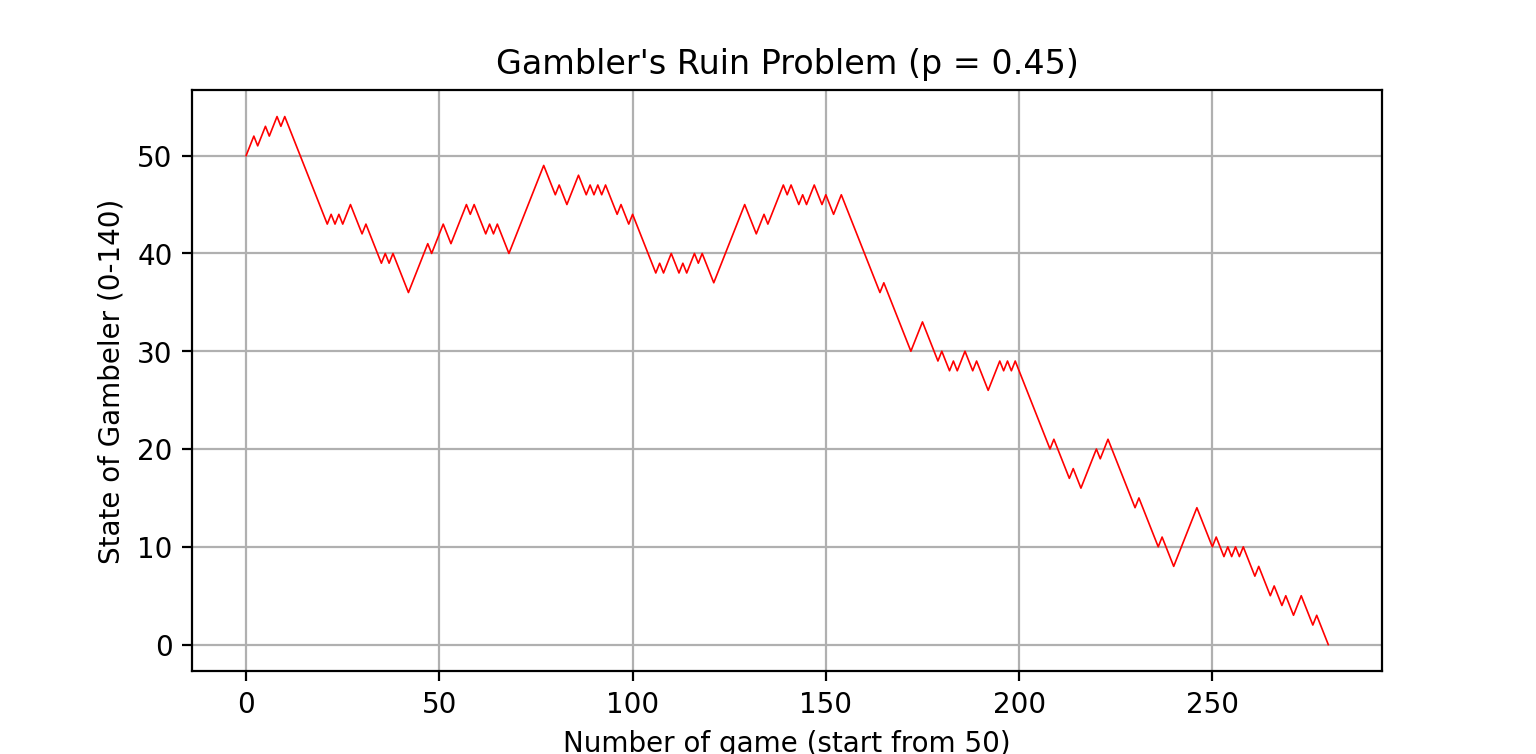
\includegraphics[width=0.8\textwidth]{pic/GR0.45.png}
    \caption{Gambler's Ruin Problem with $( p=0.45 )$}
\end{figure}

\makeatletter
\setlength{\@fptop}{0pt}
\makeatother

\begin{figure}[H]
    \centering
    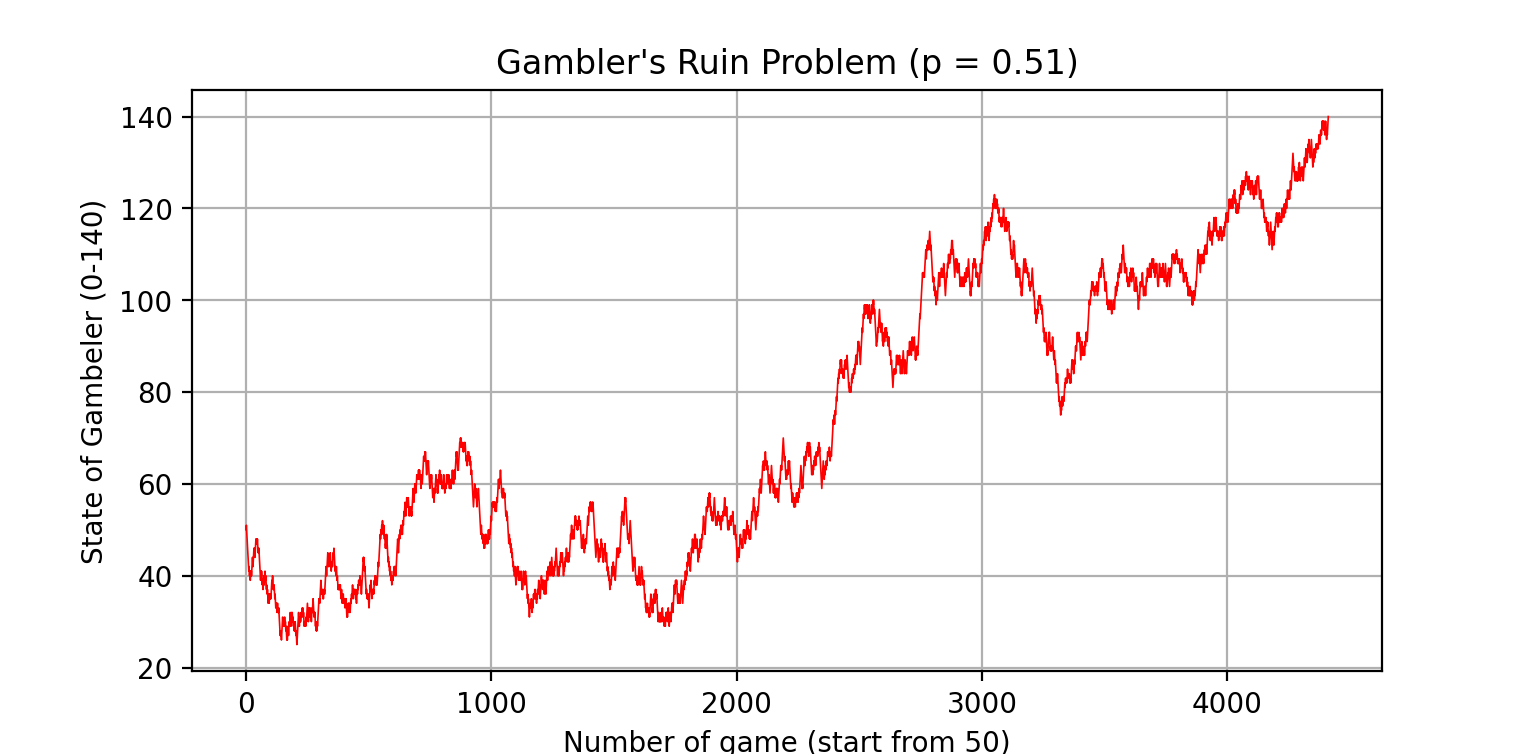
\includegraphics[width=0.8\textwidth]{pic/GR0.51.png}
    \caption{Gambler's Ruin Problem with $( p=0.51 )$}
\end{figure}

\chapter{Application of Markov Chain}
Markov chain Has  numerous application in real life. Let us explore house in this chapter.

\section{Google PageRank}
Before google surfing in the web is very hard, in search engines page was rank by primly on keyword-based algorithms to rank web pages. 
One popular early search engine, called AltaVista, used a ranking algorithm that focused on keyword matching. 
It would examine factors like the frequency of the keyword in the page's content, 
the placement of the keyword (e.g., in titles or headings), and the number of times the keyword appeared in the page's metadata.
Keyword-based algorithm is very easy to misuse. A spam page could boost its ranking
just by including a long list of words repeated over and over again.

In other hand taking the link structure into account led to dramatic improvements
in search engines. As a first attempt, one could rank a page based on how many
other pages link to it. That is, if Page A links to Page B, we consider it a “vote”
for B, and we rank pages based on how many votes they have.
But this is again very open to abuse: a spam page could boost its ranking by creating
thousands of other spam pages linking to it.
And though it may seem democratic
for each page to have equal voting power, an incoming link from a reliable page is
more meaningful than a link from an uninformative page.

To solve this problem Sergey Brin and Larry Page develop a algorithm to rank page
in their search engine Google and named it after Larry Page Google PageRank, 
which was introduced in 1998. Google PageRank ranks
the importance of a page not only by how many pages link to it, but also by the
importance of those pages.

To under stand Google PageRank we consider a smaller version of World Wide Web 
contain only 4 pages connected as shown in \cref{A small Web Containing 4 page}.

\begin{figure}[H]
    \centering
    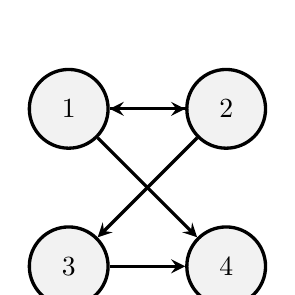
\begin{tikzpicture}[->, >=stealth, auto, very thick, node distance = 2cm, state/.style={circle, draw=black, fill=black!5, very thick, minimum size = 10mm}]
        \node[state] (1) {$1$};
        \node[state] (2) [right of=1] {$2$};
        \node[state] (3) [below of=1] {$3$};
        \node[state] (4) [below of=2] {$4$};

        \path (1) edge [] (2)
            (2) edge [] (1)
            (1) edge [] (4)
            (2) edge [] (3)
            (3) edge [] (4);
    \end{tikzpicture}
    \caption{A small Web Containing 4 page}
    \label{A small Web Containing 4 page}
\end{figure}

Imagine someone randomly surfing the web, starting at some page and 
then randomly click to get from one page to the next (with equal probabilities for
all links on the current page).
 The idea of PageRank is to measure the importance
of a page by the long-run fraction of time spent at that page.

Of course, some pages may have no outgoing links at all, such as page 4 above. When
the web surfer encounters such a page, rather than despairing he or she opens up a
new browser window and visits a uniformly random page. Thus a page with no links
is converted to a page that links to every page, including itself. For the example
above, the resulting transition matrix is

\[
    P =
    \begin{bmatrix}
        0 & 1/2 & 0 & 1/2 \\ 
        1/2 & 0 & 1/2 & 0 \\ 
        0 & 0 & 0 & 1 \\
        1/4 & 1/4 & 1/4 & 1/4
    \end{bmatrix} 
\]

If we start with probability vector 
$ \mathbf{t} = \begin{bmatrix}
    1/4 & 1/4 & 1/4 & 1/4 
\end{bmatrix}  $.\\ 
i.e. every page has equal probability to visit in first state. Then the 2nd step 
probability vector will be 
$\mathbf{t}_{1}= 
    \begin{bmatrix}
        0.1875 & 0.1875 & 0.1875 & 0.4375 
    \end{bmatrix} 
$.\\ 
Now doing $ \mathbf{t}_{2}P $ we get the 3rd step probability vector $ \mathbf{t}_{3} $.
After reputing this process we get.
\[
    \mathbf{t}_{100} \approx \mathbf{t_{101}} = \begin{bmatrix}
        0.2 & 0.2 & 0.2 & 0.4 
    \end{bmatrix} 
\]
Hence it is the stationary probability.

In general let $ M $ be the number of pages on the web, let  $ P $ be the  $ M\times M $
transition matrix of the chain described above, and 
let $ \pi $ be the stationary distribution.
Think of $ \pi_{j} $ as a measure of how important Page $j$ is. 
Hence the equitation 
\[
    \pi_{j}=\sum_{i=0}^{M} \pi_{i}p_{ij}
\]
says that the score of Page $j$ should be based not only on how many other pages link
to it, but on their scores.

It is not clear that a unique stationary distribution exists for this chain, 
since it may not be irreducible and aperiodic. 
Even if it is irreducible and aperiodic, convergence
to the stationary distribution could be very slow since the web is so immense. To
address these issues, suppose that before each move, the web surfer flips a coin
with probability $ \alpha $ of Heads. If Head, the web surfer click to a random 
link from the current page; if Tails, the web surfer teleports to uniformly random \
page. The resulting chain has the \textit{Google transition matrix}

\begin{equation}
    \label{google transition matrix}
    G = \alpha P + (1-\alpha) \frac{J}{M},
\end{equation}

where $ j $ is the  $ M\times M $ matrix of all entries are 1. Note that the row sums 
of $ G $ are 1 and that all are positive, so  $ G$ is valid transition matrix for an 
irreducible, aperiodic Markov Chain. Which means that it has unique stationary 
distribution $ \pi $, called \textit{PageRank} and the chain is converge to it.
 
The choice of $\alpha$ is an important consideration; 
choosing $ \alpha $ close to 1 makes sense to respect the structure of the
web as much as possible, but there is a tradeoff since it turns out that smaller
values of $ \alpha $ make the chain converge much faster. 
As a compromise, the original recommendation of Brin and Page was $\alpha = 0.85$.

PageRank is conceptually nice, but computing it sounds extremely difficult, considering
that that $ \pi G=\pi $ could be a system of 100 equations in 100 billion unknowns.
Instead of thinking of this as a massive algebra problem, we can use the Markov
chain interpretation: for any starting distribution  $ \mathbf{t} $,  
$\mathbf{t}G^{n}\to \pi$ as $ n\to\infty $. And $ \mathbf{t}G $ is is easier to 
compute that it seems at first:
 \[
     \mathbf{t}G = \alpha(\mathbf{t}P) +\frac{1-\alpha}{M}(\mathbf{t}J),
\]
where computing the first term is easy to compute as most element $ P $  is 0 and 
computing the second term is very easy $ \mathbf{t}J $ is a vector of all 1. 
To compute $ \mathbf{t}G^{n} $ by $ (((\mathbf{t}G)G)\ldots) $. After a very long 
iteration of $ n $ if it appear to convergent then we say  it is the approximation
of PageRank.

For the above example 
\[
    \mathbf{t}_{10000}\approx\mathbf{t}_{10001} = 
    \begin{bmatrix}
        0.2004008 & 0.2004008 & 0.2004008 & 0.3987976 
    \end{bmatrix} 
\]
Hence it is approximate Stationary Distribution.

\section{Text Generator}
Markov Chain is used in language modeling, text generation, and speech recognition. Google search, Google’s Smart Compose on Gmail are just a few examples.
Using the probabilistic properties of Markov chains to generate new text based on patterns observed in a given training text.

\textbf{Here a basic outline of how to build a text generator using the markov chain:}
\begin{itemize}
    \item \textbf{Data Processing:} Start by preparing your training text data. 
        Remove any unnecessary characters or formatting and split the text into individual nodes.
    \item \textbf{Building the Transition Matrix:} Using the given data construct the transition matrix that represent the probability to go 
        one node to another node.
    \item \textbf{Generating New Text:} To generate random text start with the initial node and Using transition matrix select the next node. 
        Repeating this we are able to generate a text.
\end{itemize}

Using the complete work William Shakespeares as a sample I able to make a text generator in python using the concept of Markov chain. Here is some output:

\begin{tcolorbox}[colback=white, colframe=black, sharp corners, boxrule=0.5pt, left=10pt, right=10pt, top=10pt, bottom=10pt]
    \small{COMMERCIALLY. PROHIBITED COMMERCIAL DISTRIBUTION INCLUDES BY ANY SERVICE THAT CHARGES FOR DOWNLOAD TIME OR USED COMMERCIALLY. PROHIBITED COMMERCIAL DISTRIBUTION INCLUDES BY}
\end{tcolorbox}

\begin{tcolorbox}[colback=white, colframe=black, sharp corners, boxrule=0.5pt, left=10pt, right=10pt, top=10pt, bottom=10pt]
    Stones have seen More free thee without more bondage happy, my cousin's hands, and is but it will come; for pulling
\end{tcolorbox}

\begin{tcolorbox}[colback=white, colframe=black, sharp corners, boxrule=0.5pt, left=10pt, right=10pt, top=10pt, bottom=10pt]
Dead shepherd, tell you live. But canst not for fashion of more turn their ends Of the worst of thunder heard
\end{tcolorbox}

\section{Other Applications}
Markov chain has very wide range of usefulness. It has use case in many fields like Data Science, AI (Artificial Intelligence), Finance etcetera.

\begin{enumerate}
    \item \textbf{Image and Signal Processing:}  Markov Random Field  a type of Markov chain, are used in image segmentation, denoising, and object recognition. 
        MRF models capture the spatial dependencies between neighboring pixels or image regions.
    \item \textbf{Finance and Economics:} Markov chains are used in modeling financial markets and analyzing economic systems. 
        it can be used to model stock prices, interest rates, and exchange rates. Markov models are also used for portfolio optimization and risk analysis.
    \item \textbf{Queueing Theory:} Markov chains are extensively used in the study of queueing systems. 
        it helps analyze the behavior of waiting lines, arrival and service processes, and queue lengths. 
        Applications include traffic engineering, telecommunications, and service operations.
    \item \textbf{Artificial Intelligence and Machine Learning:} Markov chains are utilized in reinforcement learning algorithms, 
        where an agent learns to make decisions based on a sequence of states and actions. 
        Markov decision processes (MDPs) and partially observable Markov decision processes (POMDPs) are used in planning and decision-making problems.
    \item \textbf{Genetics and Molecular Biology:} Markov chains are used to model and analyze biological sequences, such as DNA and protein sequences. 
        it is used in sequence alignment algorithms, predicting protein structures, and identifying hidden patterns in genomic data. 
\end{enumerate}

\nocite{*}
\bibliographystyle{plain}
\bibliography{ref}
\appendix
\chapter{Random Walk in Python}
\begin{figure}[H]
    \centering
    \lstinputlisting{python_scripts/RandomWalk.py}
    \caption{Random Walk python script}
    \label{RandomWalp python script}
    \centering
\end{figure}

\chapter{The Gambler’s Ruin Problem}
\begin{figure}[H]
    \centering
    \lstinputlisting{python_scripts/GamblerRuind.py}
    \caption{Gambler Ruin problem python script}
    \label{GamblerRuind python script}
\end{figure}

\chapter{Google PageRank}
\begin{figure}[H]
    \centering
    \lstinputlisting{python_scripts/GooglePageRank.py}
    \caption{Google PageRank Small simulation}
    \label{PageRank}
\end{figure}
\begin{figure}[H]
    \centering
    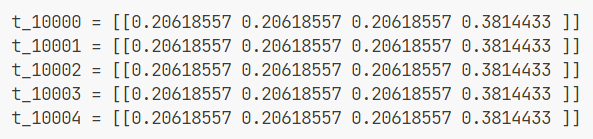
\includegraphics[width=0.6\textwidth]{pic/output of PageRank.png}
    \caption{OutPut of Google PageRank Small simulation}
    \label{OutPut Of GooglePageRank}
\end{figure}

\chapter{Text Generator}
\begin{figure}[H]
    \centering
    \lstinputlisting{python_scripts/text_sim.py}
    \caption{Text Generator using markov chain}
    \label{fig:}
\end{figure}

\end{document}
